\section{Production and information processes}

Porter's concept of information intensity and IT diversity helps explain how different industries rely on information and technology:
\begin{enumerate}
    \item Information intensity refers to the amount and complexity of information required in an organization's processes. 
     Generally, service industries require higher information intensity than manufacturing.
    \item IT Intensity measures how well IT systems meet an organization's information processing needs. 
        IT intensity is higher in banking than in insurance due to the industry's reliance on real-time transactions and data analysis.
        However, IT intensity can sometimes be greater in manufacturing than in services, depending on automation and digital integration.
    \item Management inclination reflects how much a company's leadership views IT as a strategic asset. 
        This varies based on factors like digital literacy, organizational culture, and company history.
        Historically, manufacturing companies have adopted IT earlier, while service industries experienced a lag of around ten years.
\end{enumerate}

\paragraph*{Information technology drivers}
Several factors determine how IT-intensive a company or industry can be:
\begin{enumerate}
    \item \textit{Structure of information processes}: the more structured and rule-based an activity is, the easier it is to automate using IT.
    \item \textit{Data volume}: the sheer amount of information that needs to be processed influences IT requirements.
    \item \textit{Operational frequency}: tasks that are repeated frequently benefit more from IT automation.
    \item \textit{Computational complexity}: simpler processes are easier to digitize and automate efficiently.
\end{enumerate}

\paragraph*{Porter's value chain}
Porter’s value chain concept highlights how IT supports various business activities to create competitive advantages.
\begin{figure}[H]
    \centering
    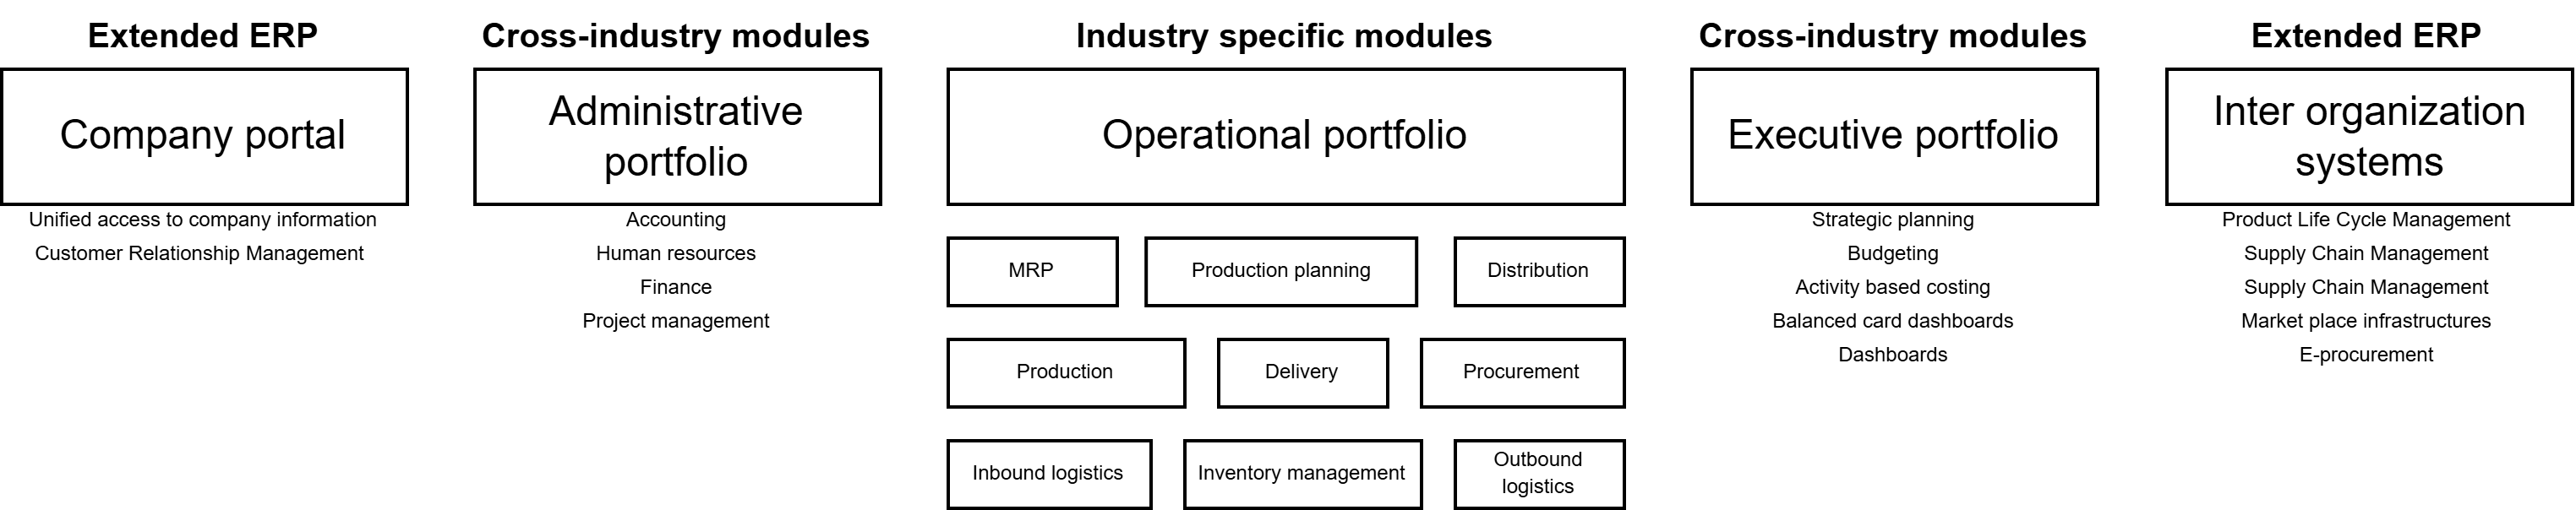
\includegraphics[width=0.5\linewidth]{images/bis1.png}
    \caption{Porter value chain}
\end{figure}

\paragraph*{Activity cycles}
Manufacturing involves continuous, iterative cycles that ensure efficiency and product quality. 
These cycles include:
\begin{enumerate}
    \item \textit{Development cycle}: focuses on designing and industrializing both products and production processes.
    \item \textit{Logistics cycle}: manages customer orders through:
        \begin{itemize}
            \item \textit{Procurement}: acquiring and handling materials, including reception, warehousing, and distribution to production plants.
            \item \textit{Production}: the physical transformation of raw materials into finished goods.
            \item \textit{Sales and distribution}: managing orders, external logistics, and post-sale services such as maintenance and customer support.
        \end{itemize}
\end{enumerate}

\subsection{Interfunctional information processes}
Interfunctional information processes play a key role in managing various aspects of production and operations within a company. 
The order management process oversees the flow of information from order check-in to post-sale services, ensuring that all customer orders are properly tracked and fulfilled. 
The materials management process handles the movement of materials, from outgoing orders to suppliers to their use in production processes. 
Similarly, the operations management process tracks the dispatching of materials to production plants and the eventual delivery of finished products.

These processes are interconnected across different products and divisions within the organization, making the information systems closely tied to the organizational structure. 
All production processes rely on the exchange of information across different functions. 
Similarly, sales activities create order information that is shared with both production and internal logistics teams.

The use of interfunctional information extends beyond production and operations into planning and control processes, such as strategic production planning, budget allocation, and scheduling. 
It also plays a vital role in administrative tasks like cash flow management and project management, helping ensure efficient resource allocation and operational success.

When considering production types, companies may engage in standard or custom production. 
Standard production involves producing items with a fixed set of features that can be modified based on customer preferences (such as color or size).
In this model, companies often produce goods according to a sales plan before receiving actual orders. 
On the other hand, custom production is driven by specific customer requirements, where production only begins once an order is confirmed.

\section{Standard and cutom products}
While custom and standard production represent opposite ends of the production spectrum, there is a continuum between the two. 
Custom production is often seen in complex products, while standard production is associated with simpler goods. 
However, the complexity of a product and its degree of standardization are independent, and all possible combinations exist.
Information technology (IT) supports all production types, although its functionalities vary depending on the degree of customization or standardization in the production process.